\documentclass[usenames,dvipsnames,pdftex,unicode,hidelinks]{beamer}

%%%%%%%%%%%%%%%%%%%%%%%%%%%%%%%
% PACKAGES
%%%%%%%%%%%%%%%%%%%%%%%%%%%%%%%

\usepackage{ucs}
\usepackage[utf8x]{inputenc}
\usepackage[english,russian]{babel}

\usepackage{eulervm} % use Euler VM font for math

\usepackage{ifdraft}

\usepackage{xspace}

\usepackage{algpseudocode}
\newcommand{\algorithmictitle}[1]{\hspace{8mm}\textbf{#1}}

\usepackage{cancel}

\usepackage{../../common/cypokcommon}

%%%%%%%%%%%%%%%%%%%%%%%%%%%%%%%
% DOCUMENT-SPECIFIC COMMANDS
%%%%%%%%%%%%%%%%%%%%%%%%%%%%%%%

% Provide some basic information about current Git revision.
%
% TODO: merge with gitinfo package?
% http://www.ctan.org/tex-archive/macros/latex/contrib/gitinfo

\InputIfFileExists{../../common/gitinfo-data}{}{
  % defaults
  \newcommand{\GitMissing}{(no Git info)}
  \newcommand{\GitAbbrHash}{\GitMissing}
  \newcommand{\GitDate}{\GitMissing}
  \newcommand{\GitSubject}{\GitMissing}
}



% add frame number to footline
\newcommand*\oldmacro{}
\let\oldmacro\insertshorttitle
\renewcommand*\insertshorttitle{
  \oldmacro\hfill
  \insertframenumber\,/\,\inserttotalframenumber
}

\newcommand{\java}{\eng{Java}\xspace}

\newcommand{\M}{\ensuremath{\mathbf{M}}}

\newcommand{\type}[1]{\mathsf{#1}}
\newcommand{\field}[1]{\mathsf{#1}}
\newcommand{\sfield}[2]{\type{#1}.\field{#2}}

\newcommand{\op}[1]{\mathbf{#1}}
\newcommand{\pts}[1]{\widebar{#1}}

%%%%%%%%%%%%%%%%%%%%%%%%%%%%%%%
% SLIDES FORMAT
%%%%%%%%%%%%%%%%%%%%%%%%%%%%%%%

\usetheme{Warsaw}
\usecolortheme{seahorse}

\setbeamercovered{transparent}

%%%%%%%%%%%%%%%%%%%%%%%%%%%%%%%
% BODY
%%%%%%%%%%%%%%%%%%%%%%%%%%%%%%%

\title[Анализ указателей и синонимов]{
  Применение анализа указателей и синонимов
  для оптимизации многопоточных программ
}
\author[Парфиненко Владимир Владимирович]{
  Парфиненко Владимир Владимирович
  \texorpdfstring{%
    \\
    \vspace{0.5cm}
    \small
      Научные руководители:\\
      м.\,н.\,с.~ИСИ~СО~РАН, Павлов~Павел~Евгеньевич \\
      зав.\,лаб.~ИСИ~СО~РАН, к.\,т.\,н.~Шелехов~Владимир~Иванович
  }{}% short title in pdf
}
\institute{
  Новосибирский Государственный Университет
}
\date{
  Новосибирск, 2013\ifdraft{ \\\medskip \footnotesize Git date: \GitDate.}{}
}

\begin{document}

\begin{frame}
  \titlepage
\end{frame}

\begin{frame}{Анализ синонимов и указателей}

  \begin{block}{Анализ синонимов \engdef{Alias Analysis}}
    Могут ли два разных выражения ссылочного типа указывать на одно и то же
    место в памяти?
  \end{block}

  \begin{block}{Анализ указателей \engdef{Points-To Analysis}}
    На какие объекты в памяти могут указывать выражения ссылочного типа?
  \end{block}

\end{frame}

\begin{frame}{Цель и задачи}

  \begin{itemize}
    \item \textbf{Цель:}
          разработка алгоритма анализа указателей для языка \java
    \medskip
    \item \textbf{Основные задачи:}
      \begin{itemize}
        \item изучить существующие алгоритмы и разработать новый, выбрав
              подходящий за основу
        \item разработать схему выражения неявных зависимостей по памяти
      \end{itemize}
  \end{itemize}

\end{frame}

\begin{frame}{Недостатки предыдущей работы}

  \begin{block}{Отсутствие чувствительности к потоку управления при работе с
      полями объектов}
    \begin{algorithmic}[1]
      \State $x \gets \op{new}~\type{T}$
      \State $x.f \gets \op{new}~\type{Object}$
      \State $a \gets x.f$
      \State $x.f \gets \op{new}~\type{Object}$
      \State $b \gets x.f$
    \end{algorithmic}
  \end{block}

  \medskip
  \centerline{\large $a$ и $b$~--- синонимы?}
  \centerline{Для алгоритма анализа, нечувствительного к потоку управления~---
  да!}

\end{frame}

\begin{frame}{Суть нечувствительного к потоку управления анализа}

  \centerline{Видение программы анализом, который к потоку управления \ldots}

  \begin{columns}[t]
    \begin{column}{0.5\textwidth}
      \begin{block}{\ldots чувствителен}
        \begin{algorithmic}[1]
          \State $x \gets \op{new}~\type{T}$
          \State $x.f \gets \op{new}~\type{Object}$
          \State $a \gets x.f$
          \State $x.f \gets \op{new}~\type{Object}$
          \State $b \gets x.f$
        \end{algorithmic}
      \end{block}
    \end{column}
    \begin{column}{0.5\textwidth}
      \begin{block}{\ldots нечувствителен}
        \begin{algorithmic}
          \State $x \gets \op{new}~\type{T}$
          \State $x.f \gets \op{new}~\type{Object}$
          \State $x.f \gets \op{new}~\type{Object}$
          \State $a \gets x.f$
          \State $b \gets x.f$
        \end{algorithmic}
      \end{block}
    \end{column}
  \end{columns}

\end{frame}

\begin{frame}{\M"=переменная}

  \begin{block}{Программа с \M"=переменной}
    \begin{algorithmic}[1]
      \State $u \gets \op{getfield}(\M_0, a, \field{f})$
        \Comment $u \gets a.\field{f}$
      \If{\ldots}
        \State $\M_1 \gets \op{putfield}(\M_0, a, \field{f}, x)$
          \Comment $a.\field{f} \gets x$
      \Else
        \State $\M_2 \gets \op{putfield}(\M_0, a, \field{f}, y)$
          \Comment $a.\field{f} \gets y$
      \EndIf
      \State $\M_3 \gets \op{phi}(\M_1, \M_2)$
      \State $v \gets \op{getfield}(\M_3, a, \field{f})$
        \Comment $v \gets a.\field{f}$
    \end{algorithmic}
  \end{block}

\end{frame}

\begin{frame}{Примитивные операции}

  \begin{columns}[t]
    \begin{column}{0.5\textwidth}
      \begin{align*}
        &\M_1 \gets \op{putfield}(\M_0, a, \field{f}, x) \\
        &\M_1 \gets \op{putstatic}(\M_0, \sfield{T}{f}, x) \\
        &\M_0 \gets \op{initialmemory } \\
        &\M_1 \gets \op{escape}(\M_0, a_1, \ldots, a_N) \\
        &\M_1 \gets \op{reload}(\M_0) \\
        &\M_x \gets \op{phi}(\M_1, \ldots, \M_N) \\
      \end{align*}
    \end{column}
    \begin{column}{0.5\textwidth}
      \begin{align*}
        &x \gets \op{getfield}(\M_0, a, \field{f}) \\
        &x \gets \op{getstatic}(\M_0, \sfield{T}{f}) \\
        &x \gets \op{shared}(\M_0) \\
        &x \gets \op{null } \\
        &x \gets \op{new}(\type{T}) \\
        &x \gets \op{phi}(a_1, \ldots, a_N) \\
      \end{align*}
    \end{column}
  \end{columns}

\end{frame}

\begin{frame}{Абстрактные объекты}

  \begin{block}{Разные источники объектов}
    \begin{algorithmic}[1]
      \State $x \gets \op{new}(\type{T})$
        \Comment $\pts{x} = \{O_1\}$
      \State $y \gets \op{new}(\type{T})$
        \Comment $\pts{y} = \{O_2\}$
      \State $u \gets \op{getstatic}(\M_0, \sfield{T}{f})$
        \Comment $\pts{u} = \{O_{global}\}$
      \State $v \gets \op{getstatic}(\M_0, \sfield{T}{g})$
        \Comment $\pts{v} = \{O_{global}\}$
    \end{algorithmic}
  \end{block}

\end{frame}

\begin{frame}{Граф операций}

  \begin{columns}[t]
    \begin{column}[T]{0.67\textwidth}
      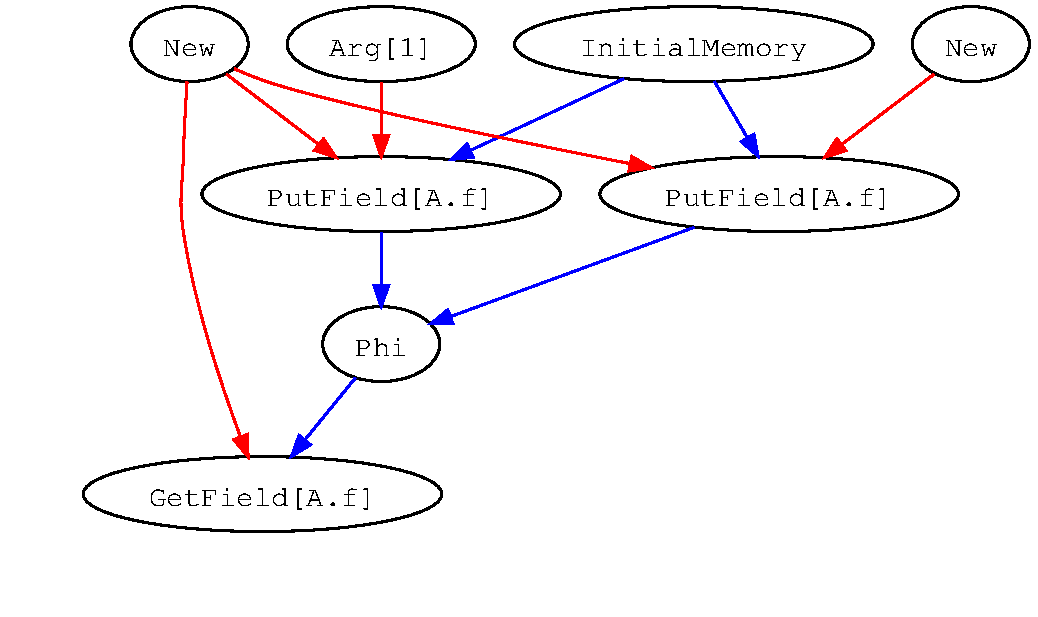
\includegraphics[width=\textwidth]{refmem_graph}
    \end{column}
    \begin{column}[T]{0.33\textwidth}
      \begin{block}{\java программа}
        \begin{algorithmic}[1]
          \State $a \gets \op{new}(\type{A})$
          \If{\ldots}
            \State $a.\field{f} \gets \op{new}(\type{A})$
          \Else
            \State $a.\field{f} \gets \op{arg}(1)$
          \EndIf
          \State $\op{return}(a.\field{f})$
        \end{algorithmic}
      \end{block}
    \end{column}
  \end{columns}

  \medskip
  \centerline{\small Красные стрелки~--- зависимость по значению.}
  \centerline{\small Синие стрелки~--- зависимость по памяти.}

\end{frame}

\begin{frame}{Алгоритм анализа}

  \textbf{Алгоритм анализа:}
  \begin{enumerate}
    \item построение вспомогательного внутреннего представления
    \item проведение потокового анализа на множестве примитивных операций
  \end{enumerate}

  \medskip
  \textbf{Результаты анализа:} \\
  выражения ссылочного типа $a$ и $b$ являются синонимами тогда и только тогда,
  когда их множества целей имеют непустое пересечение

\end{frame}

\begin{frame}{Модель памяти языка Java}
  \begin{columns}[t]
    \begin{column}{.5\textwidth}
      \begin{block}{Чтение из \eng{volatile} поля}
        \begin{algorithmic}
          \State $a.\field{x} \gets 42$
          \State $\ldots$
          \State $t \gets b.\field{volatileField}$
          \State $\ldots$
          \State $x \gets a.\field{x}$
        \end{algorithmic}
      \end{block}
    \end{column}
    \begin{column}{.5\textwidth}
      \begin{block}{Чтение из обычного поля}
        \begin{algorithmic}
          \State $a.\field{x} \gets 42$
          \State $\ldots$
          \State $t \gets b.\field{normalField}$
          \State $\ldots$
          \State \only<1>{$x \gets a.\field{x}$}
                 \only<2>{$\cancel{x \gets a.\field{x}} \Rightarrow x \gets 42$}
        \end{algorithmic}
      \end{block}
    \end{column}
  \end{columns}
\end{frame}

\begin{frame}{Практические результаты}

  \begin{itemize}
    \item<1-> Алгоритм анализа реализован в статическом компиляторе \java
              байткода в рамках проекта \eng{Excelsior Research Virtual
              Machine}.
    \item<1-> Реализованы следующие оптимизации:
          \begin{itemize}
            \item<2-> удаление избыточных чтений полей
            \item<4-> взрыв объектов и аллокация объектов на стеке
          \end{itemize}
  \end{itemize}

  \begin{columns}[t]
    \begin{column}{0.5\textwidth}
      \begin{block}{Избыточные чтения}<2->
        \begin{algorithmic}[1]
          \State $x.\field{f} \gets 42$
          \State $y.\field{f} \gets 37$
          \State \only<-2>{$u \gets x.\field{f}$}
                 \only<3->{$\cancel{u \gets x.\field{f}} \Rightarrow u \gets 42$}
        \end{algorithmic}
      \end{block}
    \end{column}
    \begin{column}{0.5\textwidth}
      \begin{block}{Взрыв объектов}<4->
        \begin{algorithmic}[1]
          \only<-4>{
            \State $r \gets \op{new}(\type{Rect})(a, b)$
            \State $u \gets r.\op{area}()$
          }
          \only<5->{
            \State $\cancel{r \gets \op{new}(\type{Rect})(a, b)}$
            \State $\cancel{u \gets r.\op{area}()} \Rightarrow u \gets a \cdot b$
          }
        \end{algorithmic}
      \end{block}
    \end{column}
  \end{columns}

\end{frame}

\begin{frame}{Результаты}

  Сделано следующее:
  \begin{itemize}
    \item изучены существующие алгоритмы анализа указателей и синонимов
    \item разработана схема выражения неявных зависимостей по памяти с помощью
          \M"=переменной
    \item разработан алгоритм, проводящий нечувствительный к потоку анализ над
          множеством операций, работающих с \M"=переменной
    \item реализован алгоритм в рамках проекта \eng{Excelsior
          Research Virtual Machine}
  \end{itemize}

\end{frame}

\begin{frame}{Дальнейшая работа}

  Планируется сделать следующее:
  \begin{itemize}
    \item внедрить в промышленный компилятор \eng{Excelsior JET}
    \item адаптировать для межпроцедурного анализа
  \end{itemize}

\end{frame}

\begin{frame}

  \centerline{\huge Спасибо за внимание!}

\end{frame}

\end{document}

